\documentclass[fleqn,10pt]{wlscirep}
\usepackage[utf8]{inputenc}
\usepackage[T1]{fontenc}
\usepackage{newfloat}
\DeclareFloatingEnvironment{video}
\title{Direction-Selective Resistance to Cerebrospinal-Fluid Flow As
the Generative Mechanism of Syringomyelia}

\author{Han Soo Chang, M.D.}
\affil{Department of Neurosurgery, Tokai University\\Isehara, Japan}

\keywords{syringomyelia, pathophysiology, simulation}
%%%%%%%%%%%%%%%%%%%%%%%%%%%%%%%%%%%%%%%%%%%%%%%%%%%%%%%%%%%%%%%%%%%%%%%%%%%%%%
% \embedvideo{<poster or text>}{<video file (MP4+H264)>}
% \embedvideo*{...}{...}                     % auto-play
%%%%%%%%%%%%%%%%%%%%%%%%%%%%%%%%%%%%%%%%%%%%%%%%%%%%%%%%%%%%%%%%%%%%%%%%%%%%%%

\usepackage[bigfiles]{pdfbase}
\ExplSyntaxOn
\NewDocumentCommand\embedvideo{smm}{
  \group_begin:
  \leavevmode
  \tl_if_exist:cTF{file_\file_mdfive_hash:n{#3}}{
    \tl_set_eq:Nc\video{file_\file_mdfive_hash:n{#3}}
  }{
    \IfFileExists{#3}{}{\GenericError{}{File~`#3'~not~found}{}{}}
    \pbs_pdfobj:nnn{}{fstream}{{}{#3}}
    \pbs_pdfobj:nnn{}{dict}{
      /Type/Filespec/F~(#3)/UF~(#3)
      /EF~<</F~\pbs_pdflastobj:>>
    }
    \tl_set:Nx\video{\pbs_pdflastobj:}
    \tl_gset_eq:cN{file_\file_mdfive_hash:n{#3}}\video
  }
  %
  \pbs_pdfobj:nnn{}{dict}{
    /Type/RichMediaInstance/Subtype/Video
    /Asset~\video
    /Params~<</FlashVars (
      source=#3&
      skin=SkinOverAllNoFullNoCaption.swf&
      skinAutoHide=true&
      skinBackgroundColor=0x5F5F5F&
      skinBackgroundAlpha=0
    )>>
  }
  %
  \pbs_pdfobj:nnn{}{dict}{
    /Type/RichMediaConfiguration/Subtype/Video
    /Instances~[\pbs_pdflastobj:]
  }
  %
  \pbs_pdfobj:nnn{}{dict}{
    /Type/RichMediaContent
    /Assets~<<
      /Names~[(#3)~\video]
    >>
    /Configurations~[\pbs_pdflastobj:]
  }
  \tl_set:Nx\rmcontent{\pbs_pdflastobj:}
  %
  \pbs_pdfobj:nnn{}{dict}{
    /Activation~<<
      /Condition/\IfBooleanTF{#1}{PV}{XA}
      /Presentation~<</Style/Embedded>>
    >>
    /Deactivation~<</Condition/PI>>
  }
  %
  \hbox_set:Nn\l_tmpa_box{#2}
  \tl_set:Nx\l_box_wd_tl{\dim_use:N\box_wd:N\l_tmpa_box}
  \tl_set:Nx\l_box_ht_tl{\dim_use:N\box_ht:N\l_tmpa_box}
  \tl_set:Nx\l_box_dp_tl{\dim_use:N\box_dp:N\l_tmpa_box}
  \pbs_pdfxform:nnnnn{1}{1}{}{}{\l_tmpa_box}
  %
  \pbs_pdfannot:nnnn{\l_box_wd_tl}{\l_box_ht_tl}{\l_box_dp_tl}{
    /Subtype/RichMedia
    /BS~<</W~0/S/S>>
    /Contents~(embedded~video~file:#3)
    /NM~(rma:#3)
    /AP~<</N~\pbs_pdflastxform:>>
    /RichMediaSettings~\pbs_pdflastobj:
    /RichMediaContent~\rmcontent
  }
  \phantom{#2}
  \group_end:
}
\ExplSyntaxOff
%%%%%%%%%%%%%%%%%%%%%%%%%%%%%%%%%%%%%%%%%%%%%%%%%%%%%%%%%%%%%%%%%%%%%%%%%%%%%%

\begin{abstract}

    The pathophysiology of syringomyelia is not well understood. The main
    theoretical problem unaddressed by previous hypotheses is how
    cerebrospinal fluid (CSF) enters from low-pressure subarachnoid space
    to high-pressure syrinx and remains inside. We approached this problem
    with a computer simulation of the CSF flow in the spine. We
    hypothesized that to-and-fro movement of CSF across a
    direction-selective resistance, via the pressure drop caused by the
    resistance, pumps the CSF in the intraspinal channel distally.

    We constructed a model of CSF dynamics in the spine, which was an
    electric circuit based on a lumped parameter model with multiple
    compartments. The model assumed a CSF channel inside the spinal cord.
    With this model, we could analyze the to-and-fro CSF movement of the
    spine. We then created a direction-selective resistance in the
    subarachnoid space. We changed a subarachnoid resistor so that it would
    resist only to the caudally-directed flow.

    In the caudal flow phase, flow across the replaced resistor produced a
    pressure drop in the distal subarachnoid segment. It subsequently
    decreased the spinal-channel pressure in the distal segment; thus, the
    pressure gradient across the point increased. This increased pressure
    gradient pumped the CSF in the channel caudally. Because this
    phenomenon did not occur in the rostral flow phase, the rostral flow in
    the channel during this phase was smaller.  Overall, each cycle of
    to-and-fro CSF movement pumped some CSF caudally in the spinal channel.

    We could reasonably hypothesize that to-and-fro CSF movement across a
    direction-selective resistance was the generative mechanism of
    syringomyelia.


\end{abstract}
\begin{document}

\flushbottom
\maketitle
% * <john.hammersley@gmail.com> 2015-02-09T12:07:31.197Z:
%
%  Click the title above to edit the author information and abstract
%
\thispagestyle{empty}


\section*{Introduction}

The pathophysiology of syringomyelia is still poorly understood. Many
hypotheses exist in the literature \cite{gardner1958mechanism,
williams1980pathogenesis, milhorat1999chiari, ball1972pathogenesis,
klekamp2002pathophysiology, duboulay1974mechanism, heiss1999elucidating,
milhorat1993anatomical, stoodley2000pathophysiology, terae1994increased,
chang2003hypothesis, chang2004theoretical, greitz2006unraveling}, but they
provide widely different explanations on the mechanisms of syrinx
generation. We may, however, enumerate what few consensuses as follows.
First, the syrinx fluid is identical to the CSF, and there is some
communication between the syrinx and the subarachnoid space. Many studies
support this point \cite{ellertsson1969syringomyelia,
ellertsson1969myelocystographic, li1987conventional, heiss2019origin},
albeit some different opinions \cite{greitz2006unraveling,
koyanagi1997surgical}. Second, some derangement of CSF flow in the spinal
subarachnoid space causes syrinx both in Chiari-I malformation
\cite{wolpert1994chiari, bhadelia1995cerebrospinal, heiss1999elucidating,
hofmann2000phasecontrast, quigley2004cerebrospinal} and subarachnoid
arachnopathy \cite{klekamp1997treatment, brodbelt2003altered,
heiss2012pathophysiology, chang2014dorsal}. Notably, the cerebellar tonsil
deranges the CSF flow in the former and adhesive arachnoiditis in the
latter.

The problem, however, is where this communicating channel resides and what
mechanism generates the syrinx. On these points, there is no solid
experimental or clinical evidence, and the opinions of researchers vary
widely. Gardner et al. \cite{gardner1958mechanism} thought that the central
canal intercommunicates the syrinx and the fourth ventricle. Arterial
pulses then exert pressure waves on the central canal and generate the
syrinx. Williams et al. also postulated the communication through the
central canal. He, however, emphasized the craniospinal pressure gradient
produced by Valsalva maneuver et al. \cite{williams1980pathogenesis}.

On the other hand, Ball and Dayan \cite{ball1972pathogenesis} assumed that
CSF entered the syrinx through the perivascular space of arteries
penetrating the spinal cord. This idea has the following variations. Heiss
et al.  \cite{heiss1999elucidating} proposed that the piston-like movement
of the cerebellar tonsils in Chiari-I patients generated pressure waves in
the spinal subarachnoid space. And it subsequently drove CSF into the
syrinx through the perivascular space. Stoodley et al. also considered the
perivascular space as the communicating channel, but he assumed the
arterial pulse pressure as the driving force \cite{stoodley2000mechanisms}.
All these assumptions are not proven and remain hypothetical. Although
recent researchers seem to favor the perivascular-space theory, there
remains the possibility that a thin communicating channel exists between
the syrinx and the fourth ventricle \cite{chang2021hypothesis}. 

In our opinion, the main theoretical problems reside in the following
points.
\begin{enumerate}
    \item No theory can explain the pathophysiological mechanism of
syringomyelia in a unified fashion.
    \item No theory can explain how CSF enters from the low-pressure subarachnoid space to the high-pressure syrinx cavity and remains inside.
\end{enumerate}

As to the first point, there are different syringomyelia types, such as
Chiari-I-malformation and spinal-arachnopathy-related
\cite{klekamp1997treatment}. The Chiari-I-malformation-related
syringomyelia is further divided into communicating and non-communicating
\cite{elliott2013syringomyelia}. Current theories cannot explain these
different types of syringomyelia in a unified fashion. However, it may be
more natural to conjecture some common mechanism underlying these different
types of syringomyelia \cite{stoodley2000mechanisms}. The second point is
theoretically essential but challenging. Physical laws dictate that the
expanded syrinx cavity has higher pressure than the subarachnoid space
\cite{serwayr.a.2016fluids, heiss1999elucidating, davis1989mechanisms,
ellertsson1970distending}, which is understandable considering the elastic
tension of the syrinx wall that the inside pressure confront. Therefore,
merely assuming a communicating channel does not explain how CSF enters the
syrinx against this pressure gradient and remains inside. Even if we take a
specific time window where the subarachnoid pressure exceeds the syrinx
pressure, it does not explain how the CSF remains inside the syrinx after
it.

The current article is part of our effort to solve the above theoretical
problems. We proposed in our previous paper \cite{chang2021hypothesis} a
hypothesis on the pathophysiology of syringomyelia. We hypothesized that a
direction-selective resistance to spinal subarachnoid CSF flow causes
syringomyelia. Suppose there is a resistance to spinal CSF flow only in
the, e.g., caudal direction. To-and-fro CSF movement across it will pump
CSF in an intraspinal channel caudally, causing syringomyelia. This
hypothesis could solve the two problems discussed above. It could solve the
paradox of CSF movement against the pressure gradient. Also, it could
explain the pathophysiology of both Chiari-I-malformation-related
syringomyelia and arachnopathy-related syringomyelia. The herniated
cerebellar tonsils function as the selective resistance in Chiari-I
malformation. And some arachnoid valve plays that role in
arachnopathy-related syringomyelia \cite{chang2014dorsal}. However, in that
article, we just drew a rough sketch of this process and left out a
detailed explanation. The current article will describe this mechanism in
detail using computer simulation.

For this purpose, we used a mathematical model simulating the CSF movement
of the spine. We revised a lumped parameter model with multiple
compartments used in our previous articles \cite{chang2003hypothesis,
chang2004theoretical}.  We placed a direction-selective resistance in this
model at a certain point in the spinal subarachnoid space. We then observed
how it affected the CSF flow in the channel inside the spinal cord.

\section*{Material and Method}

Some problem exists in the computer simulation of the motion of biological
fluids such as blood and CSF. Such bodily fluids move inside flexible
tubes. It differs from the usual situation of fluid mechanics, where the
boundary of the fluid conduit is solid. Thus, we cannot simply apply the
standard Navier-Stokes equations for our simulation. For this reason,
researchers have commonly used lumped parameter models \cite{shi2011review,
kokalari2013review}. This model considers the fluid flow inside a flexible
tube analogous to the electric flow in an electric circuit. The
accumulation of electricity in a capacitor represents the expansion of a
flexible tube and the accompanying pressure elevation. An electrical
resistor represents the frictional resistance to flow. This model has a
wide variety. For example, it may model the whole cardiovascular system as
one electric circuit, or it may model it as a synthesis of multiple
compartments of electric circuits \cite{shi2011review, kokalari2013review}.
Our current model is the type of lumped parameter model with multiple
compartments that simulates the CSF dynamics in the spine and is an updated
version of the model used in our previous articles
\cite{chang2003hypothesis, chang2004theoretical}. In this study, we did not
intend to make a quantitatively precise model of the spinal CSF flow but to
make a basic model that reveals the phenomenon underlying the generation of
syringomyelia. 

Previously, we developed a mathematical model that simulated the CSF flow
in the spine \cite{chang2003hypothesis, chang2004theoretical}. This model (a
multiple-compartment version of a 1-dimensional lumped parameter model)
could describe the CSF movement in the whole spine (Figure
\ref{fig:model}). In this model, the \textit{D} capacitors represented the
dural tension, \textit{C} capacitors the tension of the central canal,
\textit{R} resistors the frictional resistance in the subarachnoid space,
and \textit{r} resistors the frictional resistance in the central canal.

\begin{figure}[ht]
    \centering
    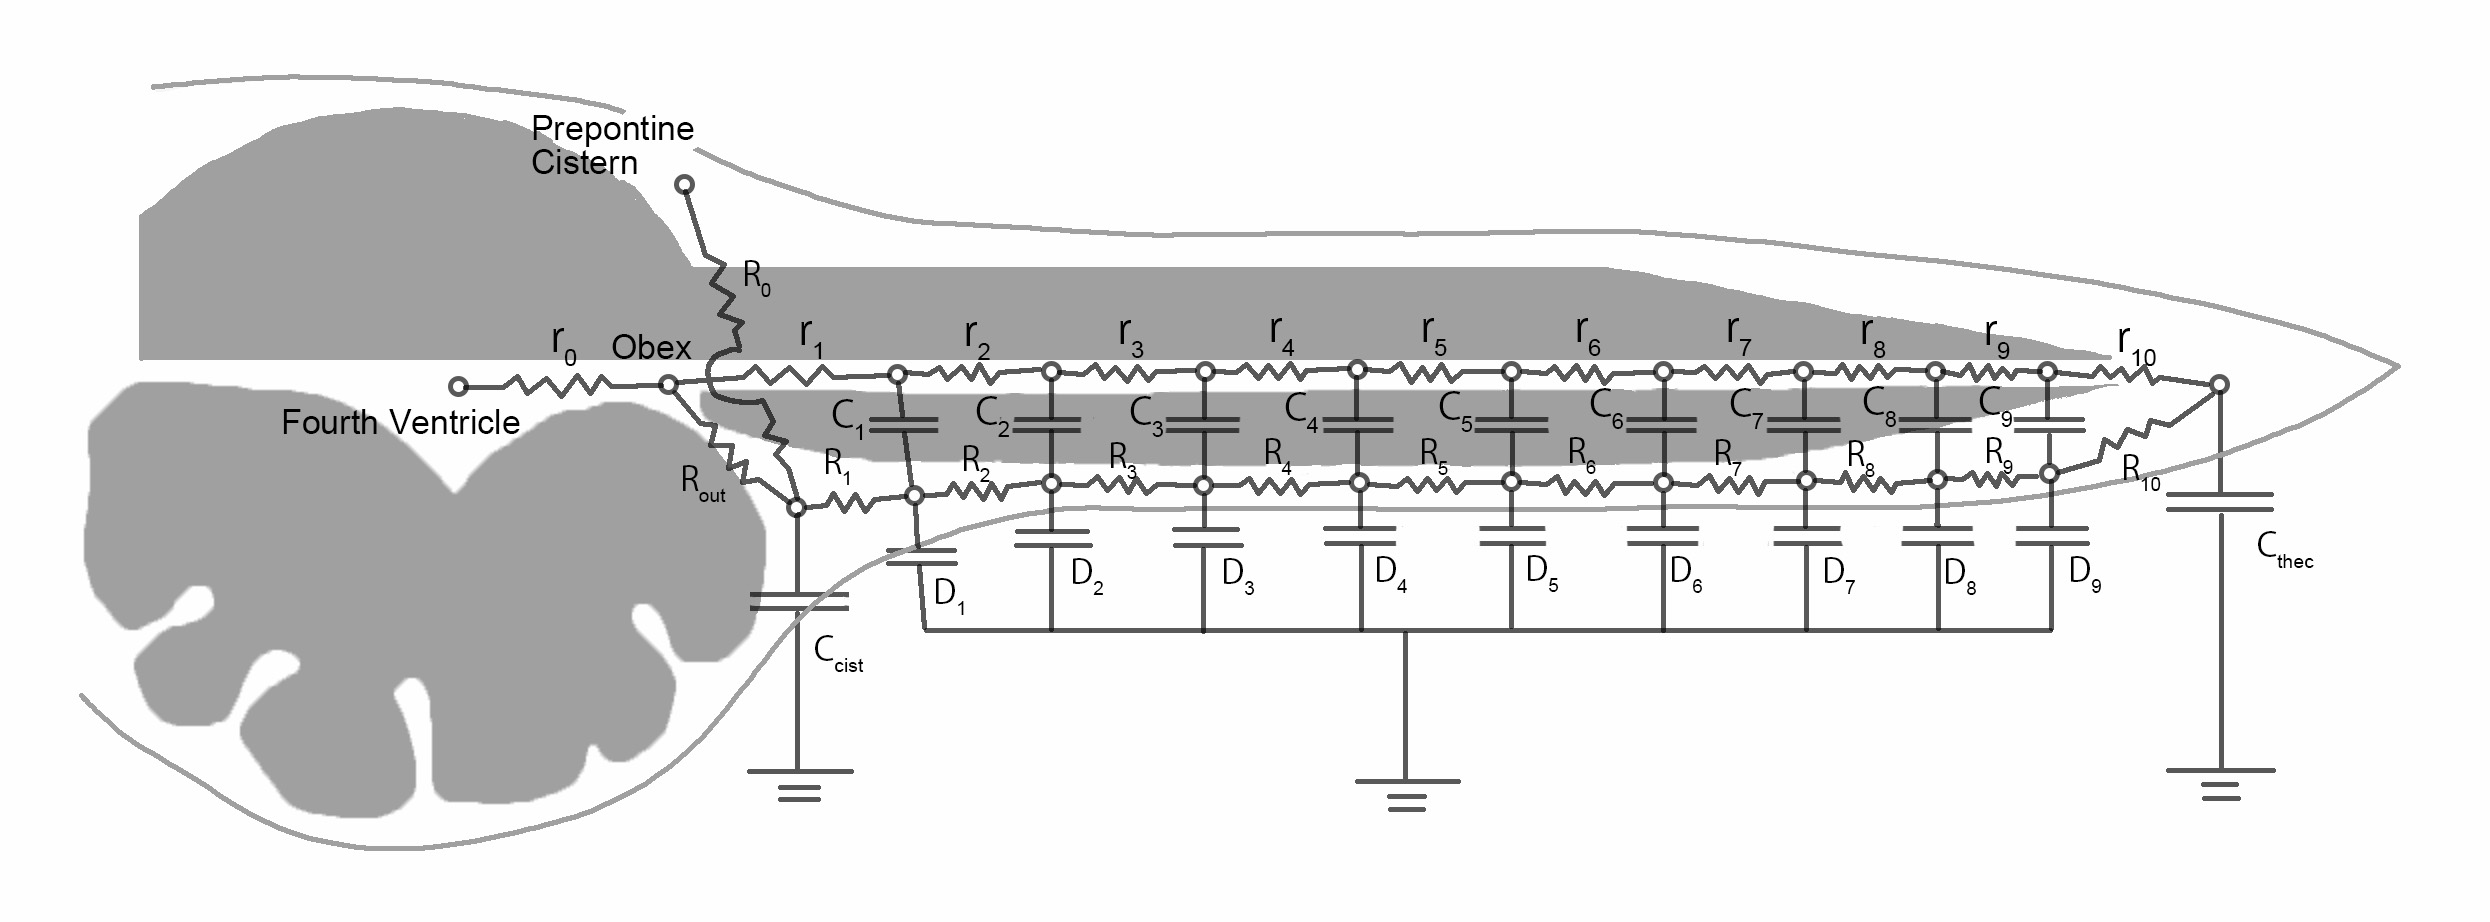
\includegraphics[width=\textwidth]{ps_circuit_schema.jpg}
    \caption{Schema of the electric circuit model of the CSF dynamics in the
    spine.}
    \label{fig:model}
\end{figure}

Figure \ref{fig:circuit} shows the bare electric circuit extracted from
Figure \ref{fig:model}. A set of differential equations could describe the
behavior of this model.  Using computer software, we could numerically
calculate its behavior in response to a certain cranial pressure wave
(defined as a boundary condition on the cranial nodes). This time, we
improved the previous model as follows.

\begin{itemize}
    \item We increased the number of compartments from 10 to 100,
        thereby making the model more precise.
    \item We revised the values of the parameters
        (the capacitance and resistance of each component)
        of the model as follows so that the model will become more realistic.
        \begin{itemize}
            \item First, we set the length of the modeled spinal cord to be 1 meter.
            \item The resistance of the subarachnoid space ($R$) was
                estimated using the following equations of Poisseuille
                \cite{brook1999numerical, sherwin2003computational, huilgol2020fast}. 
             $$\Delta P=\frac{8\pi \mu{}LQ}{A^{2}}=RQ$$
                \begin{itemize}
                    \item $\Delta P$: Pressure difference between the adjacent compartments
                    \item Q: flow speed per unit surface
                    \item $\mu$: viscosity coefficient. In this case, it was set to the value of water (0.0007).
                    \item L: distance between the adjacent compartments. It was set to 1 cm.
                    \item A: cross sectional area of the subarachnoid
                        space. It was set to the value of a concentric
                        annulus \cite{huilgol2020fast} with the outer diameter of 1cm and the inner diameter of 0.7 cm ($1.6\times{}10^{-4} (m^2)$) 
                \end{itemize}
            \item Thus, $R$ was calculated to be $6872\hspace{0.2cm}(Pa\cdot{}sec/m^3)$
            \item The resistance of the central canal ($r$) was estimated
                using the same equation with $A$ set to
                $\pi{}(10^{-4})^2\hspace{0.1cm}(m^2)$, i.e. the cross
                sectional area of a tube with a diameter of 100 $\mu{}m$.
                Thus, $r$ was calculated to be $1.78\times10^{11}\hspace{0.2cm}(Pa\cdot{}sec/m^3)$
        \end{itemize}
    \item We determined the capacitance ($C_{sub}$)corresponding to the dural elasticity so that the pressure-wave velocity determined by the time constant ($RC$) will roughly correspond to the pressure-wave velocity of the downward CSF wave observed in phase-contrast MRI of normal individuals. Thus, we set $C_{sub}=0.1\hspace{0.2cm}(m^3/Pa\cdot{}sec)$.
\end{itemize}

Figure \ref{fig:model} shows the scheme of the constructed electric circuit
model. This model represents the CSF movement in the spine as electric flow
through multiple compartments of capacitances connected with resistors.
Table 1 shows the values of the resistors and capacitors of the system. A
set of differential equations can describe the behavior of this electric
circuit, and we can solve it numerically by setting the voltage at the
cranial nodes as the boundary condition (Figure \ref{fig:circuit}). In the
previous articles \cite{chang2003hypothesis, chang2004theoretical}, we only
analyzed the transient behavior of the model to a sudden pressure increase
on the cranial side of the subarachnoid space. This analysis helped
simulate the situation of coughing or Valsalva maneuvers. In this article,
however, we analyzed the response of the model to an oscillating cranial
pressure wave simulating the normal cardiac pulsation of the CSF.

\begin{figure}[ht]
    \centering
    \includegraphics[width=\textwidth]{electric_circuit_new.jpg}
    \caption{Electric circuit diagram representing the CSF dynamics of the spine}
    \label{fig:circuit}
\end{figure}

We numerically solved the differential equations using computer software
(Mathematica version 12, Wolfram Research, Champaign, IL, U.S.A.) on a
personal computer. We set the boundary conditions as follows. (1) The
voltage at the two cranial nodes was set to a sine wave oscillating around
10 $cmH_{2}O$ with an amplitude of 20 $cmH_{2}O$ at one cycle per second.
(2) The initial dural pressure was set at 10 $cmH_{2}O$ in all segments. We
set the step of the numerical solution to 1/5000 second and calculated the
solution from zero to 20 seconds. We displayed the obtained solution as a
movie in mp4 format.

We analyzed the original normal system and two of its modifications. In the
first modification, we simply increased the subarachnoid resistance at
point 25 ($R_{25}$) by 20 times. In the second modification, we placed a
direction-selective subarachnoid resistance at point 25, so that only the
resistance to the caudal flow would be increased by 20 times.

\section*{Results}

We present the systems' responses in animations showing twenty cycles of
to-and-fro waves. The x-axis of each animation represents the 100 nodes of
the circuit laid out from the cranial to caudal direction. The y-axis
displays some of the following four measures: the dural tension (voltage in
D capacitors in Figure 2), the canal tension (voltages in C capacitors),
the subarachnoid CSF flow (flows in R resistors), and the channel flow
(flows in r resistors). We plotted the caudal flow in the positive and the
rostral flow in the negative direction. The pressure values are shown in
$cmH_2O$, the flows in $ml/sec$. To plot the four measures in a single
animation, we multiplied the following three measures---the canal tension,
the subarachnoid CSF flow, and the canal flow---with the following
coefficients, respectively: namely, the canal tension with 50, the
subarachnoid flow with 0.005, and the canal flow with $1.5\times10^{5}$. 

Video \ref{video:norm} shows the original system's response representing
the normal condition. In this state, CSF made a smooth to-and-fro movement
in the subarachnoid space with the corresponding pressure wave along the
dura and the central canal. CSF also made smooth to-and-fro movements in
the channel.

%\begin{video}[hbt]
%    \embedvideo*{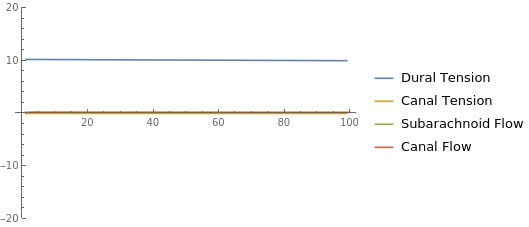
\includegraphics[width=\textwidth]{thumbnail_norm.jpg}}{totalAnimationNorm.mp4}
%    \caption{Video showing the normal circuit response}
%    \label{video:norm}
%\end{video}

In Video \ref{video:simple_block}, we increased the subarachnoid resistance
$R_{25}$ by 20 times, thereby simulating a simple block of the subarachnoid
flow in both directions. In this condition, both the caudal and rostral
flow across the resistance produced pressure drop in the distal
subarachnoid segment.  This pressure drop caused an increase in canal flow
in the same direction as the subarachnoid flow. This increased canal flow
caused a transient increase in the canal pressure distal to the block and a
decrease proximal to the block. However, these pressure changes alternated
along the alternation of the flow direction and did not produce a sustained
pressure increase.

%\begin{video}[hbt]
%    \embedvideo*{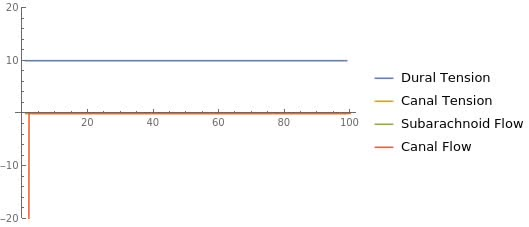
\includegraphics[width=\textwidth]{thumbnail_simple_block.jpg}}{totalAnimationSb.mp4}
%    \caption{Video showing the response of the circuit with a simple
%    resistor at point 25}
%    \label{video:simple_block}
%\end{video}
%
%\begin{video}[hbt]
%    \embedvideo*{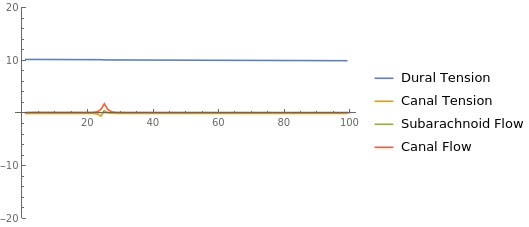
\includegraphics[width=\textwidth]{thumbnail_oneway.jpg}}{totalAnimation.mp4}
%    \caption{Video showing the response of the circuit with a
%    direction-selective resistor at point 25}
%    \label{video:oneway}
%\end{video}

%\begin{video}[hbt]
%    \embedvideo*{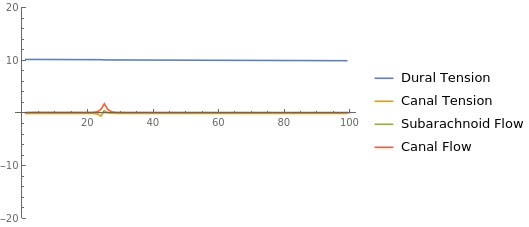
\includegraphics[width=\textwidth]{thumbnail_oneway.jpg}}{canalFlowOneway.mp4}
%    \caption{Video showing the canal flow in the model with
%    direction-selective resistance at point 25}
%    \label{video:canal_flow_oneway}
%\end{video}
%
%\begin{video}[hbt]
%    \embedvideo*{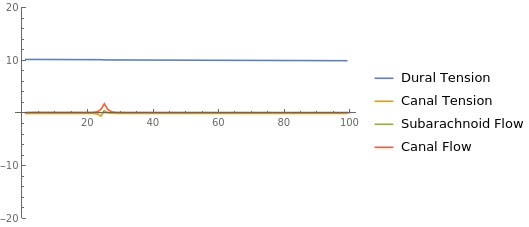
\includegraphics[width=\textwidth]{thumbnail_oneway.jpg}}{canalFlowComparison.mp4}
%    \caption{Video showing the canal flow in the two models: simple
%    resistance at point 25 and direction-selective resistance at point 25}
%    \label{video:canal_comparison}
%\end{video}

In Video \ref{video:oneway}, we replaced the subarachnoid resistor $R_{25}$
with a direction-selective resistor whose resistance to the rostral flow
was unchanged but that to the caudal flow was increased by 20 times. This
time, as shown in Video \ref{video:oneway}, sustained high pressure
appeared in the central canal in the segment distal to the replaced
resistor, and sustained low pressure in the segment proximal to it. This
sustained pressure gradually accumulated as the flow cycle proceeded. The
dural tension showed a pressure drop at node 25 only during the caudal-flow
phase. The to-and-fro canal flow increased near the node 25 similarly to
that in the simple block above, but, this time, the increase was larger in
the caudal direction.

We took out the canal flow and showed it in Video 4. Observing this video,
we can see that the cumulative total of the caudal flow is larger than that
of the rostral flow, and it means that the CSF is virtually pumped caudally
at node 25. To further elucidate this point, we plotted the canal flow in
the simple block as shown in Video \ref{video:simple_block} and that in the
one-way block as shown in Video \ref{video:oneway}. We can clearly see in
this video that the caudal flow in the canal is 


\section*{Discussion}

In this article, we theoretically analyzed the CSF movement in the spine
using a lumped parameter model with multiple components. It simulated a
system with an elastic tube (dura) containing an elastic cylindrical
material (spinal cord) that itself had a fluid channel inside (e.g. the
central canal). When we placed a direction-selective resistor in the
subarachnoid space and evoked a to-and-fro pressure wave on this system, it
produced a sustained pressure elevation in the segment distal to the
resistor in the resisted direction. This phenomenon may explain the
pathogenesis of syringomyelia both in Chiari I malformation and
syringomyelia associated with arachnopathy.

Subarachnoid pressure pushes the spinal cord material and affects the
pressure inside the central canal. As seen in Figure \ref{fig:circuit}, the
absolute pressure inside the central canal is the sum of the subarachnoid
and canal tension (voltages of $C_k$ and $D_k$ in electrical terms).
Suppose a one-way valve selectively resists caudal flow in the subarachnoid
space at point $A$. Caudal CSF flow creates a pressure drop across point
$A$, with the caudal pressure smaller than the proximal one. Thus, the
absolute pressure in the canal distal to point $A$ become smaller because
the outside subarachnoid pressure there is smaller. It, therefore, creates
a pressure gradient in the central canal across point $A$, thereby
increasing the distal CSF flow in the canal at that point (Figure
\ref{fig:pump_close}).

\begin{figure}[hbt]
    \centering
    \includegraphics[width=\textwidth]{pumping_mechanism_close.jpg}
    \caption{Increased central-canal flow across a direction-selective
    resistance in the subarachnoid space}
    \label{fig:pump_close}
\end{figure}

On the contrary, rostral flow, not encountering resistance, does not create
a pressure drop (Figure \ref{fig:pump_open}). Although some of the CSF that
had been pumped caudally during the caudal-flow phase will flow back
rostrally, its amount will be smaller. The net result will be that some CSF
is pumped caudally in one cycle of the to-and-fro movement. Thus, CSF
gradually accumulates in the distal segment of the resistance (Video 3). We
hypothesize that this is the mechanism underlying the syrinx generation.

\begin{figure}[hbt]
    \centering
    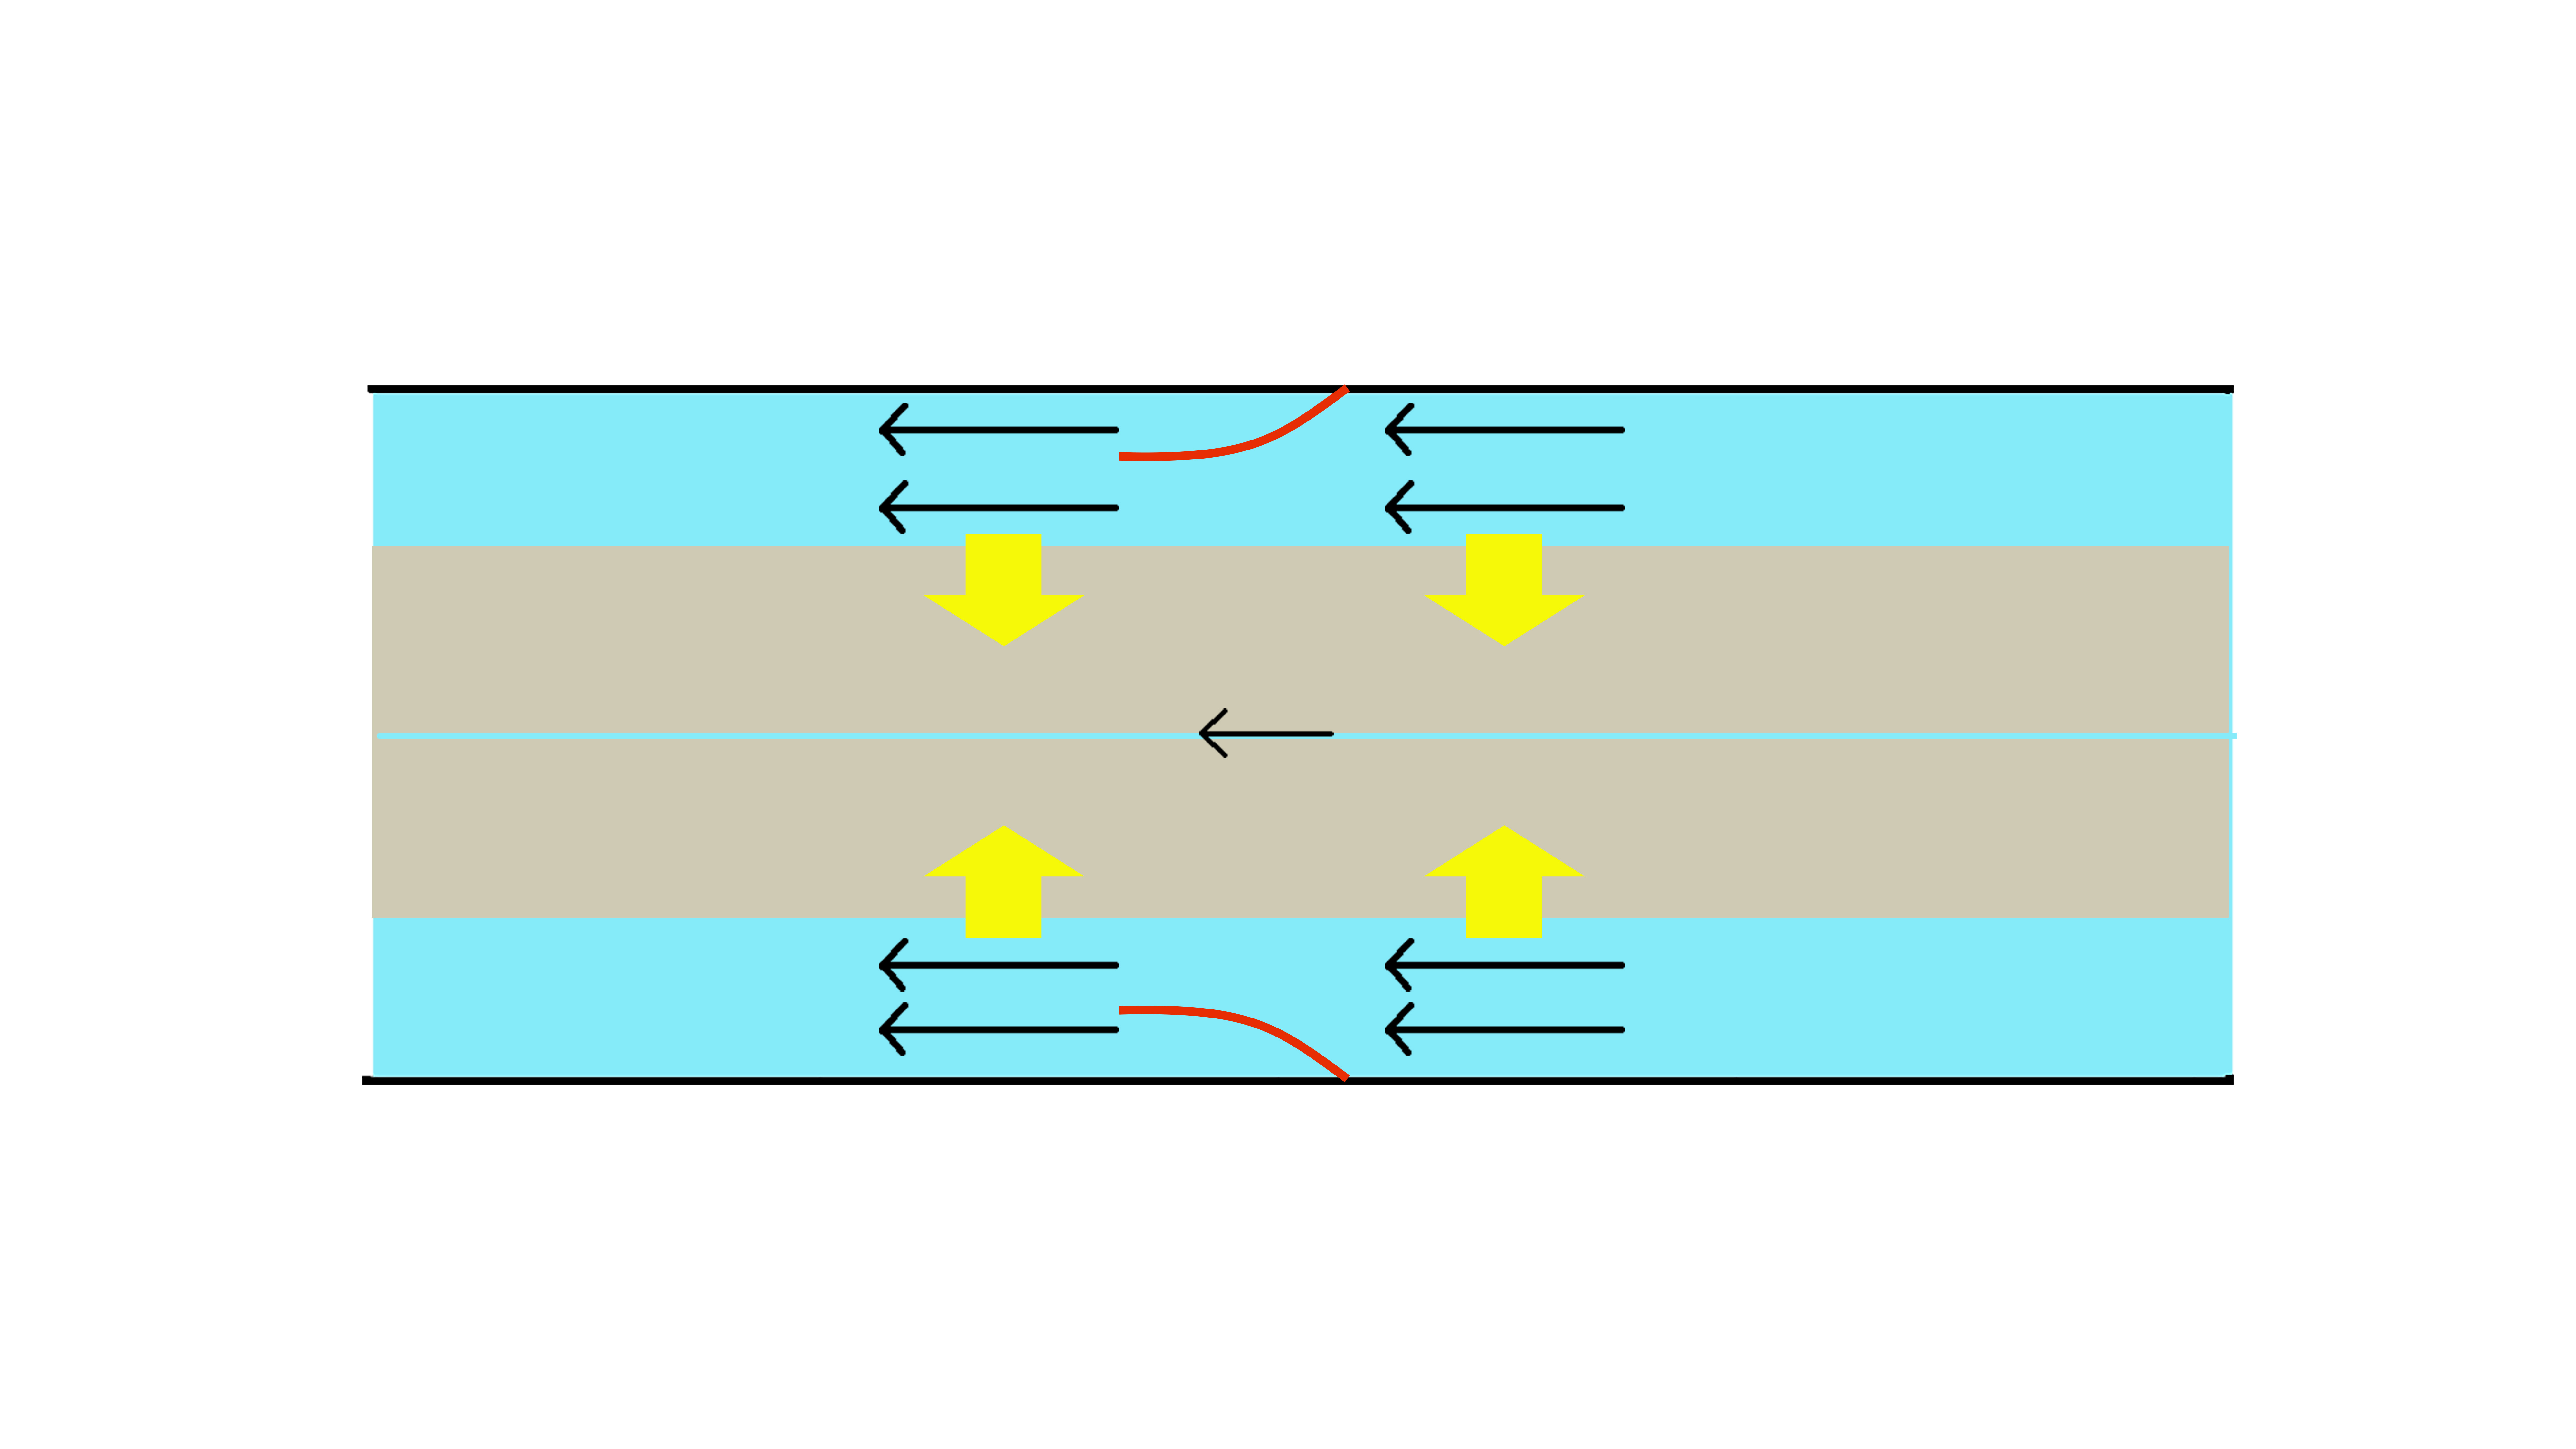
\includegraphics[width=\textwidth]{pumping_mechanism_open.jpg}
    \caption{Normal central-canal flow across a direction-selective
    resistance during the reverse flow}
    \label{fig:pump_open}
\end{figure}

This theory successfully explains how CSF is pumped against the pressure
gradient and remains inside the syrinx, one of the problems pointed out in
the Introduction. A one-way valve in subarachnoid space creates an
asymmetry of the pressure gradient between the caudal and rostral flow
phases in the central canal. This asymmetric alternation of pressure
gradient effectively pumps CSF caudally, creating sustained pressure
elevation in the caudal segment. In other words, the energy of the
to-and-fro CSF movement is translated via the one-way valve into the
creation and sustenance of syringomyelia.

Direction-selective resistance to CSF flow is not an imaginative assumption
but actually exists in patients. In Chiari-I malformation, the herniated
tonsils move like a ball-valve, displaced caudally during the caudal flow
and rostrally during the rostral flow. Higher velocity observed in the
phase-contrast MRI studies suggests that it selectively impedes the caudal
CSF flow more than the cranial flow. This direction-selective resistance
was demonstrated by Williams in direct measurements in Chiari-I patients
and became the basis of his theory \cite{williams1981simultaneous}.

Also, there is a possibility that some types of arachnoid pathology
function as one-way valves. In 2014, we reported cases of thoracic
arachnoid web associated with syringomyelia, in which phase-contrast MRI
detected one-way-valve-like behavior of the arachnoid web
\cite{chang2014dorsal}. In surgery, we found an obliquely oriented
arachnoid web that reminded us of a one-way valve. Thus, our hypothesis may
also solve the second theoretical problem we pointed out in the
Introduction. Namely, we may consider the presence of a one-way valve in
spinal subarachnoid space as a common mechanism underlying both
Chiari-I-related and arachnopathy-related syringomyelia.

Our theory clearly explained how the energy of the to-and-fro CSF movement
was transformed to CSF movement into the syrinx. However, previous
theories seemed to have difficulty in explaining this process. According to
the theories of Heiss et al. \cite{heiss1999elucidating} or that of
Stoodley et al. \cite{stoodley2000mechanisms}, the energy is provided by
either enhanced pressure waves in subarachnoid space or pulsation of spinal
arteries. However, none of these theories explains the detailed mechanism

hypothesized that arterial pulses drive CSF
into the perivascular space of the cord matrix. Although his hypothesis
explains the energy for syrinx generation, it fails to explain why
manipulation of Our theory reasonably
explained how the motion energy of the flowing CSF pumps CSF in the channel
inside the spinal cord. It is compatible with Stoodley et al.'s
experimental result that syrinx maintenance is dependent on arterial
pulsation . In this study, the authors showed that

Our restuls may cast some light on another interesting question. In
cervical spondylosis, subarachnoid space is similarly obliterated by the
protruding discs and osteophytes. Although this is a widely prevaent
disease, we rarely encounter syringomyelia associated with cervical
spondylosis. In our results, a simple block of the subarachnoid CSF flow
did not produce sustained elevation of intraspinal channel pressure (Video
\cite{video:simple_block}.  This result may explain why syringomyelia is
rarely associated with cervical spondylosis.

There are some controversial points in our theory. Our model presumed the
existence of a CSF channel inside the spinal cord. It may be controversial
because most syringes seem to lack such communication. Yet, there still may
exist a narrow CSF channel that is undetectable on MRI. In fact, ordinary
MRI does not visualize the central canal with a diameter of 100
micrometers. Therefore, assuming the existence of a CSF channel inside the
cord will not be far-fetched. Another point of controversy will be the role
of the central canal. The human central canal is obstructed with advancing
age, and assuming a function of the central canal may not befit that fact.
However, the obliteration of the central canal seem to be a slow process,
and it could be mostly patent up to the fourth decade
\cite{newman1981observations, yasui1999agerelated}. Moreover, the CSF
channel does not have to be the central canal but some other channel
created inside the spinal cord matrix.

\bibliography{my_library}


\end{document}
